\documentclass[a4paper,11pt]{report}
\usepackage[T1]{fontenc}
\usepackage[utf8]{inputenc}
\usepackage{lmodern}
\usepackage[francais]{babel}
\usepackage{graphicx}
\usepackage{array}

\title{}
\author{}

\begin{document}

\maketitle
\tableofcontents

\begin{abstract}
\end{abstract}

\chapter{Partie réseau}

\section{Modélisation des classes de réseau}

\subsection{UML de gestion des clients pour le serveur}

    \begin{figure}[th]
      \begin{center}
        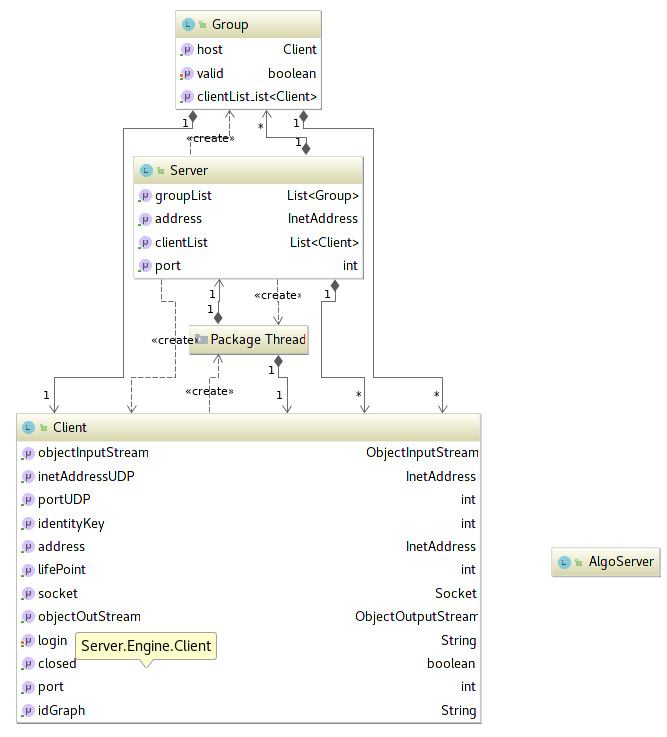
\includegraphics[scale=0.6]{Assets/UML_serveur.png}
        \caption{UML du serveur}
        \label{UML du serveur}
      \end{center}
    \end{figure}
    
    
    Comme illustré sur le diagramme ULM (\textit{figure~\ref{UML du serveur}}) le serveur contient des clients et des groupes et les groupes contiennent eux même des clients.
Un groupe possède en variable d’instance son hôte. 
Un client possède les flux objets, son socket et ses coordonnées pour le transport UDP.
Et le serveur son socket serveur TCP et UDP.





\subsection{UML de gestion des données pour les clients}
 \begin{figure}[th]
      \begin{center}
        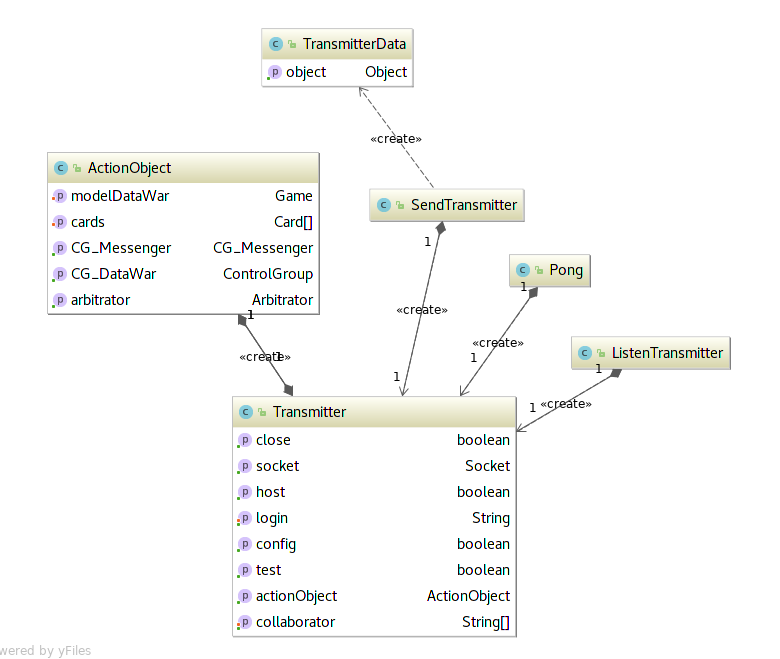
\includegraphics[scale=0.6]{Assets/UML_client.png}
        \caption{UML du client}
        \label{UML du client}
      \end{center}
    \end{figure}
    
  Comme illustré sur le diagramme ULM (\textit{figure~\ref{UML du client}}) le \textit{Transmitter} a pour variable d’instance son socket de connexion, ses flux objets, la liste des logins des membres du groupe. La variable host permet de savoir le mode hôte ou invité sur le groupe et la variable test sert aux tests logiciels. Un \textit{Transmitter} possède un \textit{ActionObject} et un \textit{ActionObject} possède un \textit{Transmitter}. La classe \textit{ActionObject} contient les contrôles groupes des applications qu’elle fait fonctionner en réseau : \textit{Messenger}, et le \textit{DataWar}.



\section{Les classes annexes}

\subsection{Visualisation de la situation du serveur}

    \begin{figure}[th]
      \begin{center}
        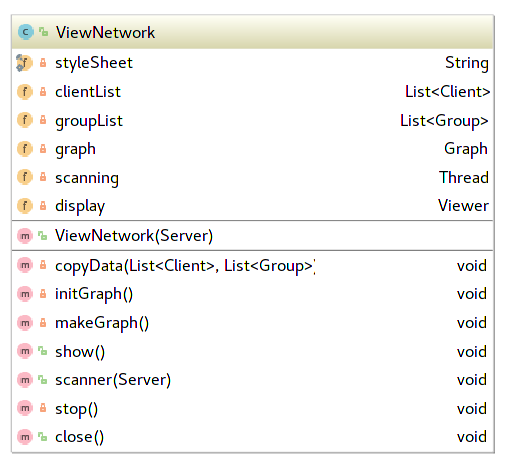
\includegraphics[scale=0.4]{Assets/UML_Network.png}
        \caption{Classe ViewNetwork}
        \label{Classe ViewNetwork}
      \end{center}
    \end{figure}
    
    La classe \textit{ViewNetwork} (Voir la \textit{figure~\ref{Classe ViewNetwork}}) permet une visualisation en temps réel de la situation du serveur. Elle montre dans une fenêtre un graphe avec pour nœud les clients et leur groupe pour liaisons. Le graphe est créé avec la librairie \textit{GraphSteam}. Lors de la création de la classe un thread est lancé pour réactualiser le graphe sur l’état du serveur. La fréquence réactualisation est de 500 millisecondes.

\subsection{Communication avec la base de donnée}

  \begin{figure}[th]
      \begin{center}
        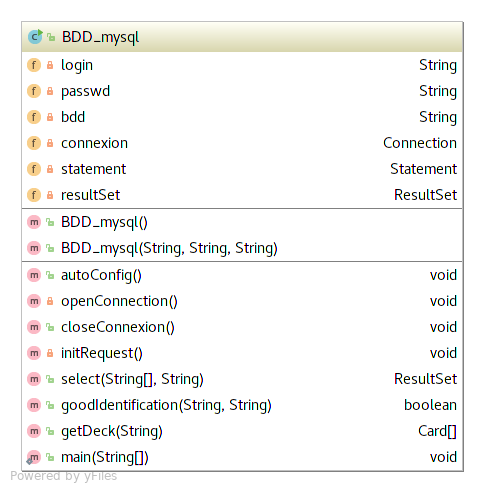
\includegraphics[scale=0.4]{Assets/UML_BDD.png}
        \caption{Classe BDD\_mysql}
        \label{Classe BDD_mysql}
      \end{center}
    \end{figure}
    
\end{document}
